\documentclass{article}
\usepackage{subcaption}
\usepackage[labelformat=parens,labelsep=quad, skip=3pt]{caption}
\usepackage{graphicx}
\usepackage[font=small,labelfont=bf]{caption}
\usepackage{geometry}

\geometry{
 a4paper,
 left=0mm,
 top=0mm,
 }

\begin{document}



\begin{figure}[htp]
 \centering
\begin{subfigure}{.33\textwidth}
 \caption{PO$_4$ - WOA (2009)}
 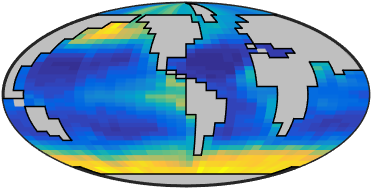
\includegraphics[width=0.95\linewidth]{../Separate_figures/OBSERVATIONS/surface_p_an.png}
\end{subfigure}%
\begin{subfigure}{.33\textwidth}
 \caption{PO$_4$ - cGEnIE}
 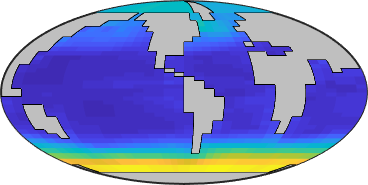
\includegraphics[width=0.95\linewidth]{../Separate_figures/BIOGEM/ocn_PO4.png}
\end{subfigure}%
\begin{subfigure}{.33\textwidth}
 \caption{PO$_4$ - EcoGEnIE}
 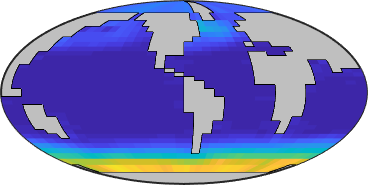
\includegraphics[width=0.95\linewidth]{../Separate_figures/ECOGEM/ocn_PO4.png}
\end{subfigure}
\\[+0.2cm]
\begin{subfigure}{.5\textwidth}
 
\includegraphics[width=0.95\linewidth]{../Separate_figures/ECOGEM/ocn_PO4_clrbr.png}
\end{subfigure}
\\
\begin{subfigure}{.33\textwidth}
 \caption{dFe - Tagliabue et al. (2012)}
 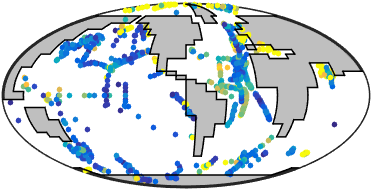
\includegraphics[width=0.95\linewidth]{../Separate_figures/OBSERVATIONS/surface_fe.png}
\end{subfigure}%
\begin{subfigure}{.33\textwidth}
 \caption{dFe - cGEnIE}
 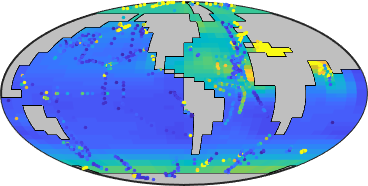
\includegraphics[width=0.95\linewidth]{../Separate_figures/BIOGEM/ocn_TDFe.png}
\end{subfigure}%
\begin{subfigure}{.33\textwidth}
 \caption{dFe - EcoGEnIE}
 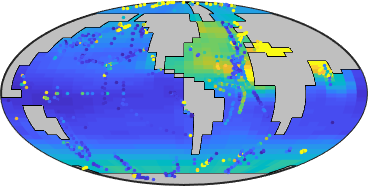
\includegraphics[width=0.95\linewidth]{../Separate_figures/ECOGEM/ocn_TDFe.png}
\end{subfigure}
\\[+0.2cm]
\begin{subfigure}{.5\textwidth}
 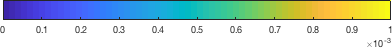
\includegraphics[width=0.95\linewidth]{../Separate_figures/ECOGEM/ocn_TDFe_clrbr.png}
\end{subfigure}
\end{figure}

\end{document}